\documentclass[twocolumn, 11pt]{article}


\usepackage{amssymb}
\usepackage{forest}
\usepackage[utf8]{inputenc}
\usepackage{import}
\usepackage{minted}
\usepackage{graphicx}
\usepackage{array}
\usepackage{tgpagella}
\usepackage{tikz}

\usepackage{newclude}
\usepackage[
backend=biber,
style=alphabetic,
sorting=ynt
]{biblatex}

\usetikzlibrary{arrows, positioning, shapes} 
\usetikzlibrary{arrows.meta}


\newtheorem{definition}{Definition}[section]
\begin{frame}
\titlepage 
\end{frame}

\begin{frame}
\frametitle{Sections} 
\tableofcontents 
\end{frame}

\addbibresource{references.bib}

\setlength{\parindent}{2em}
\setlength{\parskip}{1em}

\setlength{\columnseprule}{1pt}
\def\columnseprulecolor{\color{gray}}
\setlength{\columnsep}{1cm}

\newcommand{\writecode}[3] {
\usemintedstyle{friendly}
\begin{figure}[h!]
    \centering
    \inputminted{#1}{#2}
    \caption{#3}
\end{figure}
}

\newcommand{\code}[1]{\texttt{#1}}

\newtheorem{remark}{Utility}[subsection]
\newtheorem{corollary}{Motivation}
\newtheorem{lemma}{Assembly Connection}[subsection]

\newtheorem{observation}{Answer}[section]
\newtheorem{conclusion}{Conclusion}


\usepackage{amsmath}


\setlength\columnseprule{0pt}

\begin{document}
\maketitle

\begin{abstract}
Both monads and aspects had become a popular encapsulation method of effects into a legacy system. Programmers are increasingly using monads in their functional environments, and aspects in object-oriented settings to reduce their code's complexity and add features to their products. In this paper, we create a comparative analysis between monads and aspects, presenting their advantages and disadvantages in different contexts.
\end{abstract}

\keywords{aop, functional programming, monad, aspect, computation encapsulation}

\acm{Theory of computation}

\section{Introduction}


\begin{frame}
\frametitle{Introduction}
\framesubtitle{Motivation}
In Java, lexically scoped synchronized blocks represent the fundamental mechanism for concurrency control.
\\\\
For more flexible control, Java 5 introduced non-lexical operators, supporting locks primitives on re-entrant locks.

\begin{itemize}
    \item \texttt{ReentrantLock} class: lock and unlock operators
    \item transactional memory: onacid and commit operators
\end{itemize}
\end{frame}

\begin{frame}
\frametitle{Introduction}
\framesubtitle{Motivation}
The paper develops a \textbf{static type and effect system} to prevent the lock errors generated by improper use of those operators, for lock handling:
\begin{itemize}
    \item taking a lock without releasing it (which could lead to a deadlock)
    \item trying to release a lock without owning it
\end{itemize}
\end{frame}

\begin{frame}
\frametitle{Introduction}
\framesubtitle{Challenges}
The analysis needs to take into account the re-entrant lock's identity available at the program level, and keeps track of 
\begin{itemize}
    \item which lock is taken by which thread \item how many times it has been taken
\end{itemize}
\end{frame}

\begin{frame}
\frametitle{Introduction}
\framesubtitle{Challenges}
The analysis needs to handle three primary features: 
\begin{itemize}
    \item dynamic lock creation 
    \item passing of lock references
    \item aliasing of lock references
\end{itemize}
\end{frame}
\section{The Challenge}
\label{sec::problem}

Integrating additional computations into an existing system can shift into a difficult assignment because of the following conventional restrictions:

\begin{itemize}
    \item we are not permitted to modify a function's implementation
    \item we are not authorised to alter a function's parameters' types
    \item we are not allowed to transform the means our system composes subcomponents
\end{itemize}

Acknowledging all those limitations, one may question why such practices are necessary when mixing new services. In our examples, we limit ourselves by respecting those rules to separate our new behaviours from our legacy code. Extending our system matures into an exercise of writing new code, rather than changing existant instructions. 

Furthermore, we evaluate the general case using a mathematical model which represents our legacy context:

\begin{equation}
\begin{cases}
f_1 :: A_1 \rightarrow A_2 \rightarrow \dots \rightarrow A_n \rightarrow X_1 \\
f_2 :: B_1 \rightarrow B_2 \rightarrow \dots \rightarrow B_n \rightarrow X_2 \\
\vdots \\
f_n :: Z_1 \rightarrow Z_2 \rightarrow \dots \rightarrow Z_n \rightarrow X_n \\
h :: X_1 \rightarrow X_2 \rightarrow \dots \rightarrow X_n \rightarrow Y
\end{cases}
\end{equation}

Our model composes $n$ functions $ f_i, i = \overline{1,n} $ using $ h $, each function represents an independent computation; to simplify our model, we can consider those a set of serial processes.

Our model is composed of $n$ various functions $ f_i, i = \overline{1,n} $ and one transformation $h$ which combines all $f_i$, each mapping represents an independent computation; to simplify, we acknowledge this set of processes to be serial and synchronised.

The granted practices permit us to adjust the manner in which we apply our function $(h (f_1 a_1 \dots a_n) \dots (f_n z_1 \dots z_n))$, without altering the conclusive output. The circumstances enable us to consider two options when blending a new operation:

\begin{itemize}
    \item using dynamic detection and automatic evaluation; with an aspect which encapsulates a new process, and pointcuts which detects the target action's location in our implementation scope
    \item using static detection and automatic evaluation; with a monad to encapsulate our computation, and its bind function to evaluate it
\end{itemize}

Those two proposals tackle unique situations; by using aspects, we enlarge our implementation space from a two-dimensional setting, defined by our operation's position (where we formulate our instructions), and its time (when performing our behaviour) to a multidimensional environment, in which each distinct computation defines a dissimilar dimension of implementation. 

\begin{figure}
    \centering
    \def \spaceNode {4cm}

\tikzstyle{action} = [rectangle, rounded corners, font=\linespread{1}\selectfont,
draw, text width=4em, text badly centered, inner sep=4pt]

\tikzstyle{other} = [circle, rounded corners, font=\linespread{1}\selectfont,
draw, text width=2em, text badly centered]
            
\begin{center}
\begin{tikzpicture}[node distance=10mm]
% The axes
\draw[red, -{Latex[red,length=3mm,width=3mm]}, to path={|- (\tikztotarget)}] (xyz cs:x=0) -- (xyz cs:x=3) node[above] {$computation\#1$};
\draw[blue, -{Latex[blue,length=3mm,width=3mm]}, to path={|- (\tikztotarget)}] (xyz cs:y=0) -- (xyz cs:y=3) node[right] {$computation\#2$};
\draw[black!60!green, -{Latex[black!60!green,length=3mm,width=3mm]}, to path={|- (\tikztotarget)}] (xyz cs:z=0) -- (xyz cs:z=3) node[left] {$computation\#3$};
\end{tikzpicture}
\end{center}

    \caption{Aspect-Oriented Implementation Space}
    \label{fig::dimensions::aop}
\end{figure}

In different circumstances, monads elevate our computation into a different scope, which distinguishable to an extension is not self-supporting from the previously mentioned framework. A monad represents a pattern which uses high-level functions, mathematical functors, and comes as a solution for effect encapsulation.

\begin{figure}
    \centering
    
\begin{center}
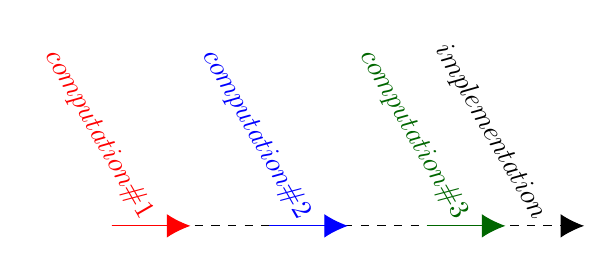
\begin{tikzpicture}[node distance=10mm]

\draw[dashed, -{Latex[black,length=3mm,width=3mm]}, to path={|- (\tikztotarget)}] (xyz cs:x=4.5) -- (xyz cs:x=10.5) node[left=5mm, rotate=-60] {$implementation$};

\draw[red, -{Latex[red,length=3mm,width=3mm]}, to path={|- (\tikztotarget)}] (xyz cs:x=4.5) -- (xyz cs:x=5.5) node[left=5mm, rotate=-60] {$computation\#1$};
\draw[blue, -{Latex[blue,length=3mm,width=3mm]}, to path={|- (\tikztotarget)}] (xyz cs:x=6.5) -- (xyz cs:x=7.5) node[left=5mm, rotate=-60] {$computation\#2$};
\draw[black!60!green, -{Latex[black!60!green,length=3mm,width=3mm]}, to path={|- (\tikztotarget)}] (xyz cs:x=8.5) -- (xyz cs:x=9.5) node[left=5mm, rotate=-60] {$computation\#3$};


\end{tikzpicture}
\end{center}
    \caption{Aspect-Oriented Implementation Space in Object-Oriented Environments}
    \label{fig::dimensions::oop}
\end{figure}

Let us examine a reduced variant of our overall intricacy, to explain each strategy using monads and aspects.

\begin{equation}
\begin{cases}
f:: Int \rightarrow String \rightarrow Boolean \\
g :: String \rightarrow Float \rightarrow Double \\
h :: Boolean \rightarrow Double \rightarrow Int
\end{cases}
\end{equation}

Although all the thoughts exhibited in our paper are self-supporting from a programming language or paradigm, we use Kotlin to produce a \textit{runnable} implementation of our clarifications for several reasons:

\begin{itemize}
    \item Kotlin is a multi-paradigm language with supports functional and object-oriented features
    \item Kotlin holds a static and powerful type system
    \item Kotlin empowers us with extensions on generic types for supplementary operations, which is useful to clarify our monad's implementation
\end{itemize}


\section{Monad's Approach}
\label{sec::solution}

Our monadic data structure operates as a wrapper which carries our extra behaviour and shrouds our original transformation's application $h(f(4, "test"), g("test", 4.0))$; the aforementioned technique holds beneficial features because it lets us to chain further operations, mixes them and later determines which calculation we evaluate at runtime. 

\writecode{java}
    {__code/monad_solution.kt}
    {Monad's generic implementation in Kotlin}
\label{fig::solution::monad::example}

This approach provides us with adaptability at the expense of loquacity; we have to improve the method of applying our function h with a less convenient lambda nesting arrangement. Some functional languages permit us to manage this behaviour with syntactic sugar such as a do notation.

\writecode{haskell}
    {__code/better.hs}
    {Alternative calling method in with do notation in Haskell}
\label{fig::better::haskell}
 
We can also decorate our initial operation with another new behaviour by using a chain of bind function calls, or we can apply our initial computation multiple times. 

\writecode{kotlin}
    {__code/composing_computation.kt}
    {Composing computations with bind function}
\label{fig::composition::monad}

Composing monads of different types with a map function will allow us to convert between the bind calls the type of additional computation we are expecting.

\begin{equation}
    map :: a \rightarrow b \rightarrow (M N a \rightarrow M N b)
\end{equation}

\begin{equation}
    map :: map_M \cdot map_N
\end{equation}

Flexibility is the primary advantage of using monads over aspects; we can easily extend our monads to generate new computation or add additional computations on top of our bind function.

\section{Aspect's Approach}
\label{sec::aop}

Aspects provide an alternative solution for our problem, in which we can control when and where the execution of our additional computation takes place.

\writecode{java}
    {__code/aop_solution.java}
    {Aspect-oriented platform independent solution}
\label{fig::aop::solution}

Depending on the programming language, aspects may provide us with a rich and powerful detection mechanism. In languages such as Java, C\#, Kotlin or Groovy, we can detect annotations and compose aspects using them on our functions, classes or properties.

Other programming languages, especially functional ones do not provide us with this type of reflection detection; we are limited to detect the location where our additional computation will execute using the function's properties such as its name, parameters types or return value type. 

Such imposed limitations make our aspects challenging to combine and extend; we have to modify our existing code, the aspect's pointcut to change the location of the execution of our new behaviour. 

Furthermore, some programming languages do not support aspects as an extension framework or standard library, so their usage is limited, unlike monad's universal usages.
 
The dynamic control of our aspect's execution, defined by its pointcut provides a powerful mechanism which allows us to add additional computations without changing our existent code (not even the application of our h function).

Unlike monads, aspects do not patch our code with additional wrappers (at least not explicitly), our compiler or interpreter takes care of the job of their coupling with our existent system.

\begin{figure}
    \centering
    \tikzstyle{action} = [rectangle, rounded corners, font=\linespread{1}\selectfont,
draw, text width=4em, text badly centered, inner sep=4pt]

\tikzstyle{other} = [circle, rounded corners, font=\linespread{1}\selectfont,
draw, text width=6em, text badly centered]
            
\begin{center}
\begin{tikzpicture}[node distance=10mm]
            
\node[action] [fill=white] (advice) {$advice$};

\node[action] [below left=7mm of advice, fill=white] (pointcut) {$pointcut$};

\node[] [below=7mm of advice] (label) {$aspect$};
\node[action] [below right=7mm of advice, fill=white] (target) {$target_B$};

\node[other] [above left=20mm and 8mm of advice] (A) {$A$};
\node[other] [above right=20mm and 8mm of advice] (B) {$B$};

\node[action] [right=-7mm of A, fill=white] (fA) {$method_A$};
\node[action] [left=-7mm of B, fill=white] (fB) {$method_B$};

\node [draw=black, dashed, fit={(advice) (pointcut) (target)}]{};

\draw[shorten >=  0cm, shorten <= 0cm, -{Latex[black,length=3mm,width=3mm]}, to path={|- (\tikztotarget)}]
(fA) edge [bend right=-30] node[above=0.2cm] {oop flow} (fB)
(fA) edge [bend right=30] node[left=0.2cm] {$joinpoint$} (advice)
(advice) edge [bend right=30] node[right=0.2cm] {aop flow} (fB);
\end{tikzpicture}
\end{center}

    \caption{Aspect-Oriented As Proxy}
    \label{fig::gateway::oop}
\end{figure}


\section{Related Work}
\label{sec::related::work}

Over the past two decades, a couple of impressive papers highlighted the connection between our two approaches. Prof. Wolfgang De Meuter's paper "Monads as a theoretical foundation for AOP" \cite{monthfoundaop} presents a set of similarities between monads and aspects, and how we can use monads in functional programming to simulate or replace the need for aspects from the aspect-oriented paradigm.

\large{\textbf{1. Aspect-oriented extensions for functional programming languages}}

An intriguing branch of the functional community tries to combine the two approaches presented in this paper into a single environment, by implementing an aspect-oriented extension for functional languages. 

A refreshing example of such a language is Aspectual Caml based on Objective Caml \cite{inproceedings}. An aspect is viewed as an extension of a given data structure and a modification of the evaluation's behaviour. 

In a functional programming language, currying functions define the structure of a given program; Aspectual Caml offers unique features such as curried pointcuts, which detect those types of functions in our code base.

\large{\textbf{2. Anticipation of effects}}

A challenging requirement in aspect-oriented code represents the anticipation of effects. In large systems controlled and manipulated by multiple aspects, it gets difficult to manually evaluate the effects produced by our functions and data structures \cite{Wang:2009:APM:1596614.1596621}.

Usually, in functional programming languages, all effects are encapsulated into monadic structures (or applicative functors or comonads) \cite{Wang:2009:APM:1596614.1596621}, adding advices into a functional program will generate a new approach in encapsulating side-effects. This addition may generate a difficulty when evaluating the time complexity of a given algorithm, and a challenging situation in lazily evaluated computations.

The predictability factor of our programs will suffer if we use both methods to encapsulate computations \cite{Wang:2009:APM:1596614.1596621}.

\section{Conclusions}

\begin{conclusion}
Dissimilar with other pipeline architectures, VTK uses executive objects to coordinate the interactions between data components and process components. This design decision creates a complex data flow infrastructure, which is difficult to analyse and trace.
\end{conclusion}

\begin{conclusion}
Despite the overall simple architecture, the rendering system is too challenging to extend. Creating a new type of filter requires detailed planning and solving multiple edge cases for distributed data and parallel execution.
\end{conclusion}


\printbibliography

\end{document}
